\documentclass{labReport}
\urlstyle{same}

\let\verbatim\undefined 
\let\verbatimend\undefined 
\lstnewenvironment{verbatim}{\lstset{breaklines,basicstyle=\ttfamily}}{}
\usepackage{lipsum}

\title{Lab 3: Iterative Algorithms}
\author{Adam Haile, Aiden Miller, Leigh Goetsch}
\prof{Dr. Berisha}
\className{Algorithms \& Adv. Data Struct.}
\classCode{CSC 3310}
\semester{Fall 2024}
\submissionDate{10/26/2024}
\labWeek{6}
\laboratoryDate{10/11/2024}

\begin{document}
\maketitle

\section*{Learning Outcomes}
\begin{itemize}
    \item Design an algorithm for a given computational problem statement
    \item Justify the correctness of an algorithm
    \item Perform asymptotic complexity analysis of the run time of an algorithm
    \item Generate test cases for an algorithm
    \item Correctly implement an algorithm from pseudocode
    \item Design and execute benchmarks for an algorithm
\end{itemize}

% if you want a TOC:
% \tableofcontents

\newpage
% if you want to use multicols:
\begin{multicols*}{2}
\raggedcolumns

For this lab we selected \\\textit{\textbf{Problem 1: Determine if a Point is Located Inside a Polygon}}.\\ The challenge is to determine whether a point lies inside or outside a polygon. The inputs are:
\begin{itemize}
    \item A sequence $<p_1, p_2, ..., p_n>$ of $n \geq 3$ 2D points.  Each point is a pair of x and y coordinates.  The points correspond to the vertices of a simple (non-intersecting) polygon.  The polygon is connected by line segments between each adjacent pair of points, including a line segment from the last point to the first point.
    \item The x and y coordinates for a single point distinct from the vertex points.
\end{itemize}
The output is:
\begin{itemize}
    \item A Boolean value indicating whether the point is located inside the polygon.
\end{itemize}

\section{Decision Rule}
% A paragraph describing a “decision rule” that can be applied to solve to the computational problem. Provide at least 2 illustrations (test cases) that demonstrate how the rule is applied.

Draw a horizontal line originating from the point infinitely to the right. 
If the number of times the line intersects with the point is odd, the point is located inside the polygon.

\begin{figure}
     \centering
     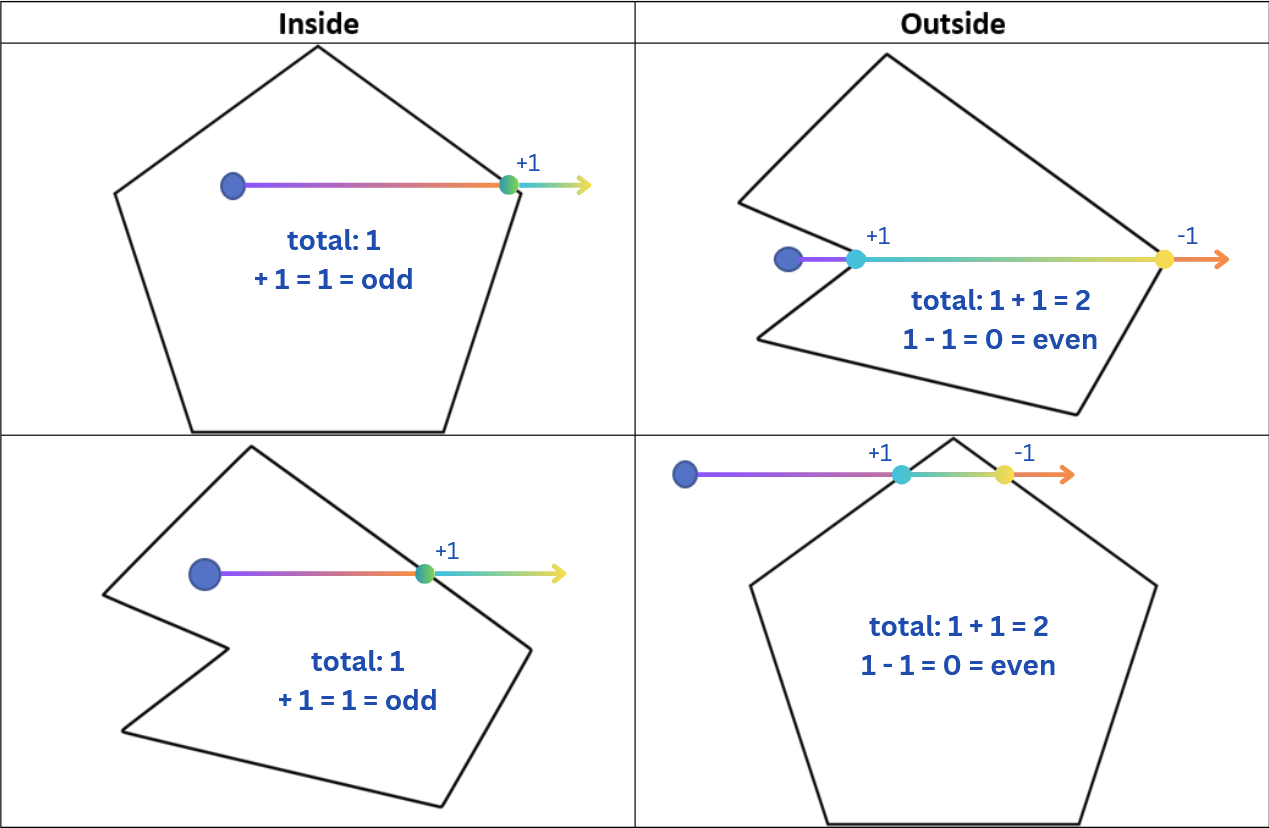
\includegraphics[width=1\linewidth]{images/decision_boundary.png}
\end{figure} 

\vspace{5em}

\section{Pseudocode}
% 2. High-level pseudocode for an algorithm that uses that rule to solve the computational problem for any input
\begin{verbatim}
inclusive = false
points = [list of polygon points]
distinct_point = (x, y)

vectors = drawVectors(points)
right_line = rightVector(distinct_point)

wn = 0
for vector in vectors:
    if counterclockwise_check(vector, right_line) or onsegment_check(vector, right_line, inclusive):
        wn += 1

return wn % 2 == 1
\end{verbatim}
\textbf{Explanation:}

\begin{itemize}
    \item For each vector, check if the line intersects. 
    \begin{itemize}
        \item If it intersects, increment. 
    \end{itemize}
    \item If the total is odd, return true.
\end{itemize}

\section{Algorithm Justification}
% 3. Provide an explanation and justification for why your algorithm is correct (1-3 paragraphs)
This algorithm is the same one as is used in the \textit{ray-casting method}. The ray-casting parity argument, which the ray-casting method solves, says that a ray from the right of a given point extended to infinity will cross an even number of lines of a polygon if it is outside, and an odd number if it is outside every time. This works because every time the ray crosses a polygon edge, it switches between being "inside" and "outside."

\section{Time Analysis}
% 4. Perform an analysis of the worst-case run time using asymptotic notation.
This algorithm exact analysis runtime is $T(n) = 105n + 6$, with a time complexity of O(n), where n represents the number of vectors which represent the polygon's edges.

\section{Test Cases}
% 5. A table of your test cases, the answers you expect, and the answers returned by running your implementation of the algorithm.
\begin{table}[H]
\centering
\begin{tabular}{|c|c|c|c|}
\hline
\textbf{Test Case} & \textbf{Shape Type} & \textbf{Test Point(s)} & \textbf{Expected Result} \\ \hline
1 & Triangle      & Polygon Center  & Inside (True) \\ \hline
2 & Square        & Polygon Center      & Inside (True) \\ \hline
3 & Pentagon      & Polygon Center      & Inside (True) \\ \hline
4 & Hexagon       & Polygon Center      & Inside (True) \\ \hline
5 & Octagon       & Polygon Center      & Inside (True) \\ \hline
6 & Triangle      & Various outside points & Outside (False) \\ \hline
7 & Square        & Various outside points & Outside (False) \\ \hline
8 & Pentagon      & Various outside points & Outside (False) \\ \hline
9 & Hexagon       & Various outside points & Outside (False) \\ \hline
10 & Octagon      & Various outside points & Outside (False) \\ \hline
11 & Concave1     & Polygon Center        & Inside (True) \\ \hline
12 & Concave2     & Polygon Center        & Inside (True) \\ \hline
13 & Concave3     & Polygon Center        & Inside (True) \\ \hline
14 & Concave4     & Polygon Center        & Inside (True) \\ \hline
15 & Concave5     & Polygon Center        & Inside (True) \\ \hline
16 & Concave1     & Inside Concavity      & Outside (False) \\ \hline
17 & Concave2     & Inside Concavity      & Outside (False) \\ \hline
18 & Concave3     & Inside Concavity      & Outside (False) \\ \hline
19 & Concave4     & Inside Concavity      & Outside (False) \\ \hline
20 & Concave5     & Inside Concavity      & Outside (False) \\ \hline
21 & Concave5     & Inside Concavity      & Outside (False) \\ \hline
\end{tabular}
\caption{Test Cases and Results for Polygon Inclusion. All Passed}
\label{tab:test_cases}
\end{table}
    

\newpage
\section{Benchmarking}
% 6. A table and graph from benchmarking your implementation on problem instances of different sizes. The benchmarks should support your theoretically derived run time.
\begin{table}[H]
\centering
\begin{tabular}{|c|c|}
\hline
\textbf{Polygon Size} & \textbf{Run Time (seconds)} \\ \hline
3    & \(3.6 \times 10^{-5}\) \\ \hline
5    & \(2.2 \times 10^{-5}\) \\ \hline
10   & \(3.8 \times 10^{-5}\) \\ \hline
50   & \(1.63 \times 10^{-4}\) \\ \hline
100  & \(3.20 \times 10^{-4}\) \\ \hline
500  & \(2.18 \times 10^{-3}\) \\ \hline
1000 & \(3.90 \times 10^{-3}\) \\ \hline
2000 & \(7.876 \times 10^{-3}\) \\ \hline
\end{tabular}
\caption{Polygon Size vs. Run Time}
\label{tab:runtime}
\end{table}



\end{multicols*}

% add appendix
% 7. Attach all your source code and test cases in an appendix.
\begin{verbatim}
from typing import List, Tuple
from pydantic import BaseModel

import matplotlib.pyplot as plt

import random as rd
import polygenerator as pg
import time
import statistics as st

rd.seed(42)

class Vector(BaseModel):
"""
Represents a vector in 2D space
"""
point_1: Tuple[float, float]
point_2: Tuple[float, float]

def get_right_line(distinct_point: Tuple[float, float]) -> Vector:
    """
    Get the infinite line that is to the right of the distinct point
    """
    return Vector(point_1=distinct_point, point_2=(float('inf'), distinct_point[1]))

def draw_vectors(points: List[Tuple[float, float]]) -> List[Vector]:
    """
    Get a list of vectors from a list of points
    """
    vectors = []
    for i in range(len(points)):
        if i == len(points) - 1:
            vectors.append(Vector(point_1=points[i], point_2=points[0]))
        else:
            vectors.append(Vector(point_1=points[i], point_2=points[(i+1)]))

    return vectors

def plot_polygon(vectors: List[Vector], right_line: Vector) -> None:
    """
    Plot the polygon vectors and the right line
    """
    for vector in vectors:
        x_values = [vector.point_1[0], vector.point_2[0]]
        y_values = [vector.point_1[1], vector.point_2[1]]
        plt.plot(x_values, y_values, marker='o')

    plt.scatter(right_line.point_1[0], right_line.point_1[1])
    plt.plot([right_line.point_1[0], min(3, right_line.point_2[0])], [
            right_line.point_1[1], right_line.point_2[1]], linestyle='--')
    # plt.xlim(-1, 2)
    # plt.ylim(-1, 2)
    plt.xlabel('X-axis')
    plt.ylabel('Y-axis')
    plt.title('Polygon Vectors')
    plt.grid(True)
    plt.show()

    def ccw(p1: Tuple[float, float], p2: Tuple[float, float], p3: Tuple[float, float]) -> bool:
    """
    Determine if three points are listed in a counterclockwise order
    Time Complexity: O(1)
    """
    return (p3[1] - p1[1]) * (p2[0] - p1[0]) > (p2[1] - p1[1]) * (p3[0] - p1[0])


def collinear(p1: Tuple[float, float], p2: Tuple[float, float], p3: Tuple[float, float]) -> bool:
    """
    Determine if three points form collinear vectors
    Time Complexity: O(1)
    """
    return (p3[1] - p1[1]) * (p2[0] - p1[0]) == (p2[1] - p1[1]) * (p3[0] - p1[0])


def on_segment(p1: Tuple[float, float], p2: Tuple[float, float], p3: Tuple[float, float]) -> bool:
    """
    Determine if a point is on a segment
    Time Complexity: O(1)
    """
    return collinear(p1, p2, p3) and min(p1[0], p2[0]) <= p3[0] <= max(p1[0], p2[0]) and min(p1[1], p2[1]) <= p3[1] <= max(p1[1], p2[1])


def intersect(v1: Vector, v2: Vector, check_edge: bool) -> bool:
    """
    Determine if two vectors intersect
    Time Complexity: O(1)
    """
    if ccw(v1.point_1, v2.point_1, v2.point_2) != ccw(v1.point_2, v2.point_1, v2.point_2) and ccw(v1.point_1, v1.point_2, v2.point_1) != ccw(v1.point_1, v1.point_2, v2.point_2):
        return True

    if check_edge and (on_segment(v2.point_1, v2.point_2, v1.point_1) or on_segment(v2.point_1, v2.point_2, v1.point_2)):
        return True

    return check_edge and (on_segment(v1.point_1, v1.point_2, v2.point_1) or on_segment(v1.point_1, v1.point_2, v2.point_2))


def inside_polygon(vectors, point, inclusive=True) -> bool:
    """
    Determine if a point is inside a polygon
    Time Complexity: O(n) where n is the number of vectors in the polygon
    """

    right_line = Vector(point_1=point, point_2=(float('inf'), point[1]))

    return sum(intersect(vector, right_line, inclusive) for vector in vectors) % 2 == 1

    points = [(0.5, 0), (0, 1.5), (1, 2.5), (2, 1.5), (1.5, 0)]

distinct_point = (1, 1)

vectors = draw_vectors(points)

vectors

right_line = get_right_line(distinct_point)
right_line

plot_polygon(vectors, right_line)
inside_polygon(vectors, distinct_point)

# Polygons
polygon_sizes = [3, 5, 10, 50, 100, 500, 1000, 2000]
polygons = [pg.random_polygon(size) for size in polygon_sizes]

# Points
points = [(rd.uniform(0, 1), rd.uniform(0, 1)) for _ in range(3)]

def benchmark_inside_polygon(polygon, point):
    """
    Benchmark the inside_polygon function
    """
    start_time = time.perf_counter()
    polygon = draw_vectors(polygon)
    inside_polygon(polygon, point)
    end_time = time.perf_counter()
    elapsed = end_time - start_time
    return elapsed

results = []
# Check if points are inside polygons
for polygon in polygons:
    point_results = []
    for point in points:
        point_results.append(benchmark_inside_polygon(polygon, point))
        # plot_polygon(draw_vectors(polygon), get_right_line(point))
    results.append(st.mean(point_results))

import numpy as np
from scipy.stats import linregress

# fit a linear regression model to the log of the list
# sizes (s) and run times (r) to estimate the slope (m)
# log r = m log s + b


def estimate_slope(list_sizes, run_times):
    '''
    Function takes a list of list sizes and a list of run times
    and returns the slope of the linear regression model.
    '''
    m, b, _, _, _ = linregress(np.log(list_sizes), np.log(run_times))
    return m


def get_complexity(m):
    '''
    Function takes the slope of the linear regression model
    and returns the complexity of the algorithm.
    '''
    if m == 0:
        return "Constant"
    elif m < 1:
        return "Sub-linear (e.g., log n)"
    elif m == 1:
        return "Linear"
    elif m > 1 and m < 2:
        return "Between linear and quadratic (e.g., n log n)"
    elif m == 2:
        return "Quadratic (e.g., n^2)"
    elif m > 2 and m < 3:
        return "Between quadratic and cubic (e.g., n^2 log n)"
    elif m == 3:
        return "Cubic (e.g., n^3)"
    else:
        return "Out of Scope"


# Validate the the formal run time complexity of the algorithms
m = estimate_slope(polygon_sizes, results)
complexity = get_complexity(m)
print(f"Estimated Slope: {m}")
print(f"Complexity: {complexity}")
print()

# Plot the results
plt.plot(polygon_sizes, results, marker='o')
plt.xlabel('Polygon Size')
plt.ylabel('Run Time (s)')
plt.title('Run Time vs. Polygon Size')
plt.grid(True)
plt.show()

def plot_vectors(vectors: List[Vector], distinct_point: Tuple[float, float] = None) -> plt.figure:
    #create figure\n",
    plt.figure(figsize=(4, 4)),
    for vector in vectors:
        x_values = [vector.point_1[0], vector.point_2[0]]
        y_values = [vector.point_1[1], vector.point_2[1]]
        plt.plot(x_values, y_values, marker='o')
    
    if distinct_point != None:
        plt.scatter(distinct_point[0], distinct_point[1])
        plt.plot([right_line.point_1[0], min(3, right_line.point_2[0])], 
             [right_line.point_1[1], right_line.point_2[1]], linestyle='--')
    plt.xlim(-1, 3)
    plt.ylim(-1, 3)
    plt.xlabel('X-axis')
    plt.ylabel('Y-axis')
    plt.title('Polygon Vectors')
    plt.grid(True)
    # return figure
    return plt.gca()

plot = True

# Test 1: Basic shapes, i.e square, triangle, pentagon, hexagon, octagon
triangle_points = [(0, 0), (1, 0), (0.5, 1)]
square_points = [(0, 0), (0, 1), (1, 1), (1, 0)]
pentagon_points = [(0.5, 0), (0, 1), (1, 2), (2, 1), (1.5, 0)]
hexagon_points = [(0, 0), (1, 0), (1.5, 0.75), (1, 1.5), (0, 1.5), (-0.5, 0.75)]
octagon_points = [(0, 0), (1, 0), (1.5, 0.5), (1.5, 1), (1, 1.5), (0, 1.5), (-0.5, 1), (-0.5, 0.5)]

square_vectors = draw_vectors(square_points)
triangle_vectors = draw_vectors(triangle_points)
pentagon_vectors = draw_vectors(pentagon_points)
hexagon_vectors = draw_vectors(hexagon_points)
octagon_vectors = draw_vectors(octagon_points)

#plot shapes
if plot:
    plot_vectors(triangle_vectors)
    plot_vectors(square_vectors)
    plot_vectors(pentagon_vectors)
    plot_vectors(hexagon_vectors)
    plot_vectors(octagon_vectors)

# Cases
# Positive case, center of polygon
test_pt = (0.5, 0.5)
assert inside_polygon(triangle_vectors, test_pt) == True
assert inside_polygon(square_vectors, test_pt) == True
assert inside_polygon(pentagon_vectors, test_pt) == True
assert inside_polygon(hexagon_vectors, test_pt) == True
assert inside_polygon(octagon_vectors, test_pt) == True

# Negative case, outside 3x3 square of points outside polygon
test_points = [(-1, -1), (1, -1), (3, -1), (3, 0.5), (3, 3), (0.5, 3), (-1, 3), (-1, 0.5)]
assert all(inside_polygon(triangle_vectors, pt) == False for pt in test_points)
assert all(inside_polygon(square_vectors, pt) == False for pt in test_points)
assert all(inside_polygon(pentagon_vectors, pt) == False for pt in test_points)
assert all(inside_polygon(hexagon_vectors, pt) == False for pt in test_points)
assert all(inside_polygon(octagon_vectors, pt) == False for pt in test_points)

cancave1 = [(1.0770230274977621, 2.0), (1.0701214824718508, 1.58083570903468), (0.0, 0.0), (2.0, 0.3280763018072074)]
cancave2 = [(2.0, 1.1750318240428033), (1.9221019042924747, 2.0), (0.44248435290975957, 1.4793109390850825), (0.0, 1.4913457706722701), (0.06830485309367998, 0.0)]
cancave3 = [(1.1353953052877837, 0.8619812579522), (0.953073457124504, 1.0174427304337217), (2.0, 1.5961192650889844), (0.41295676178745566, 2.0), (0.0, 1.414657286604214), (1.9647627125185438, 0.0)]
concave4 = [(2.0, 0.8700732229633639), (0.0, 2.0), (0.39547774682317083, 0.003916977341347422), (0.46990464802695203, 0.0), (1.475853861061979, 0.27025365835577414), (1.7612717964530658, 0.7860492477511123), (1.4969619566741321, 0.7911312296845074)]
concave5 = [(1.9999999999999998, 1.8394892346839924), (1.4342282628973673, 2.0), (0.3159937397907171, 1.5898477952887802), (0.40740519742818926, 1.1231500217492716), (0.0, 0.9281072619689151), (0.5793287716307272, 0.954722493942688), (1.2550474040617023, 0.5755607503698047), (1.3444909644895129, 0.0)]

cancave1_vectors = draw_vectors(cancave1)
cancave2_vectors = draw_vectors(cancave2)
cancave3_vectors = draw_vectors(cancave3)
concave4_vectors = draw_vectors(concave4)
concave5_vectors = draw_vectors(concave5)

#plot shapes
if plot:
    plot_vectors(cancave1_vectors)
    plot_vectors(cancave2_vectors)
    plot_vectors(cancave3_vectors)
    plot_vectors(concave4_vectors)
    plot_vectors(concave5_vectors)

# Positive case, center of polygon
test_pt = (1, 1)
assert inside_polygon(cancave1_vectors, test_pt) == True
assert inside_polygon(cancave2_vectors, test_pt) == True
assert inside_polygon(cancave3_vectors, (1, 1.5)) == True
assert inside_polygon(concave4_vectors, test_pt) == True
assert inside_polygon(concave5_vectors, test_pt) == True

# Negative case, inside the concave part of the polygon
assert inside_polygon(cancave1_vectors, (1, 1.75)) == False
assert inside_polygon(cancave2_vectors, (0.5, 1.6)) == False
assert inside_polygon(cancave3_vectors, (1.5, 1)) == False
assert inside_polygon(concave4_vectors, (1.9, 0.5)) == False
assert inside_polygon(concave5_vectors, (1, 0.5)) == False
assert inside_polygon(concave5_vectors, (0.2, 1.5)) == False
\end{verbatim}


\end{document}
